\documentclass{tietreport}
\usepackage{graphicx}
\usepackage{booktabs}
\usepackage{array}
\usepackage{enumitem}
\usepackage{tikz}
\usetikzlibrary{arrows.meta,positioning,shapes.geometric,fit}
\hypersetup{colorlinks=true,linkcolor=black,urlcolor=black,citecolor=black}

\TitlePageHeader{UCS503 - Software Engineering}
\ProjectTitle{ReplayDB}
\ProjectSubTitle{A Temporal Database Debugging and Time-Travel Replay System}
\author{Harkirat Singh}
\TitlePageSubText{BE Third Year, Computer Science and Engineering}
\AdvisorName{Department of Computer Science and Engineering}
\TitlePageFooterText{{\large Prototype Stage Report \\[0.2cm]
\bfseries Computer Science and Engineering Department}\\[0.15cm]
Thapar Institute of Engineering and Technology, Patiala}

\tikzset{box/.style={draw,rounded corners=3pt,align=center,minimum height=8mm,minimum width=28mm,fill=gray!8},actor/.style={draw,ellipse,align=center,minimum height=8mm,minimum width=25mm,fill=orange!12},arrow/.style={-Latex,thick},small/.style={font=\small}}

\begin{document}
\maketitle
\tableofcontents

\chapter{Introduction}
\section{Background and Context}
Modern applications change database records through user actions, scheduled jobs, migrations, and service integrations. When a value becomes incorrect, the current database state rarely explains what changed, who changed it, or which related records were affected. Developers commonly combine logs, backup snapshots, and ad-hoc SQL queries to investigate incidents. This is slow and can itself risk modifying production data.

ReplayDB is an educational temporal-debugging platform for PostgreSQL. It captures row-level mutations in an append-only event ledger and exposes them through an interface for forensic transaction inspection, historical replay, field-level comparison, and read-only counterfactual analysis.

\section{Problem Statement}
Given an unexpected value in a relational database, a developer needs to identify the committed transaction that caused it, inspect all affected rows, reconstruct the record at an earlier point in time, and assess the likely state if the faulty transaction had not occurred. Existing logs are often incomplete and conventional database views normally show only the latest state. ReplayDB addresses this gap through an immutable mutation ledger, deterministic reconstruction, and an explainable forensic workflow.

\section{Project Objectives}
\begin{enumerate}[label=O\arabic*.]
  \item Capture insert, update, and delete mutations with old state, new state, transaction identifier, timestamp, database user, and query context.
  \item Reconstruct a record or table state at a selected historical event without changing the live database.
  \item Group related writes by transaction to expose the blast radius of a suspected incident.
  \item Compare actual state with a counterfactual timeline in which selected transactions are omitted.
  \item Provide a clear browser workflow and validate it through automated, API, responsive, and end-to-end tests.
\end{enumerate}

\section{Scope and Limitations}
The prototype supports PostgreSQL-oriented change capture and an in-memory demonstration ledger. It is intended for controlled development and educational investigation, not production restoration. A branch is read-only: it explains a possible alternative state but does not execute a rollback. Later transactions may depend on a removed event; consequently, the default comparison is evaluated at the incident moment so the direct consequence is visible.

\chapter{Requirement Analysis}
\section{Stakeholders and Requirements}
The primary actor is a developer or database administrator investigating incorrect data. A tester uses the controlled incident scenario to verify replay behaviour. A maintainer configures monitored tables and capture triggers.

\begin{center}
\begin{tabular}{p{0.13\textwidth}p{0.75\textwidth}}
\toprule
ID & Requirement \\
\midrule
FR1 & Record row-level INSERT, UPDATE, and DELETE events in an append-only ledger. \\
FR2 & Display the chronological history of a selected table record. \\
FR3 & Reconstruct state at any captured event and show field-level differences. \\
FR4 & Group events sharing a transaction ID and show affected tables. \\
FR5 & Create a counterfactual branch excluding one or more transaction IDs. \\
FR6 & Search the ledger and manage monitored table capture. \\
\bottomrule
\end{tabular}
\end{center}

\section{Use-Case Diagram}
\begin{figure}[h]
\centering
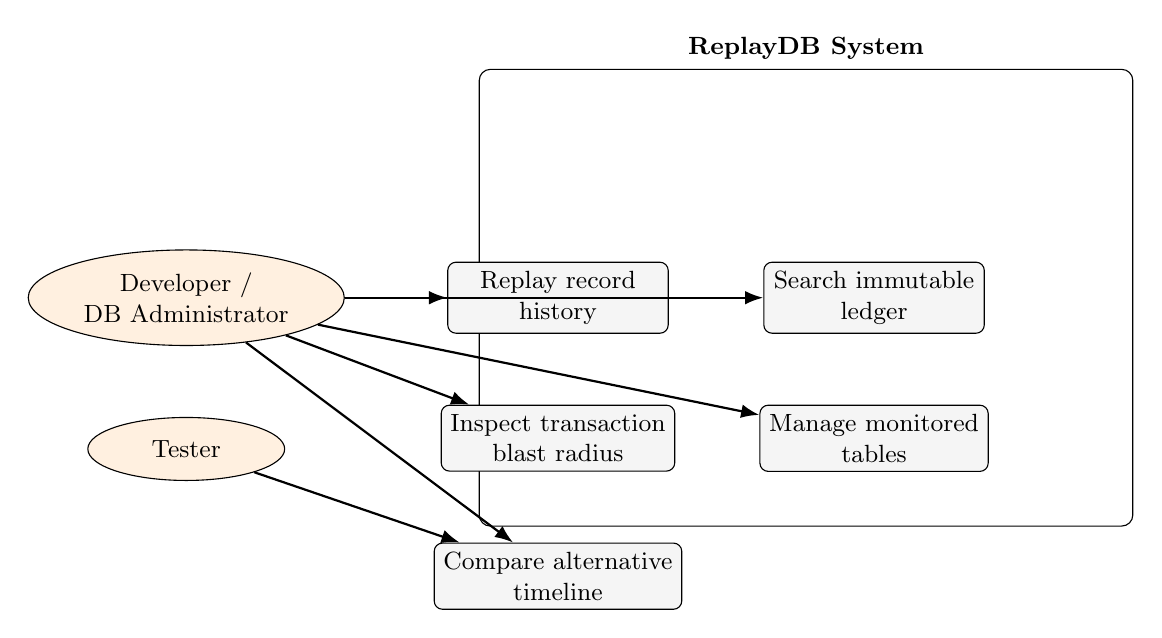
\begin{tikzpicture}[node distance=9mm and 17mm,small]
\node[actor] (dev) {Developer /\\DB Administrator};
\node[actor,below=of dev] (tester) {Tester};
\node[draw,rounded corners,minimum width=83mm,minimum height=58mm,right=of dev,label=above:{\textbf{ReplayDB System}}] (system) {};
\node[box,right=13mm of dev] (studio) {Replay record\\history};
\node[box,below=of studio] (tx) {Inspect transaction\\blast radius};
\node[box,below=of tx] (branch) {Compare alternative\\timeline};
\node[box,right=12mm of studio] (ledger) {Search immutable\\ledger};
\node[box,below=of ledger] (tables) {Manage monitored\\tables};
\draw[arrow] (dev)--(studio); \draw[arrow] (dev)--(tx); \draw[arrow] (dev)--(branch); \draw[arrow] (dev)--(ledger); \draw[arrow] (dev)--(tables); \draw[arrow] (tester)--(branch);
\end{tikzpicture}
\caption{Primary use cases for ReplayDB.}
\end{figure}

\chapter{Methodology and Design}
\section{SDLC Model}
An iterative and incremental SDLC model was selected. Each iteration delivers a vertical slice: event capture, record replay, transaction forensics, counterfactual comparison, and interface refinement. This approach suits the project because feedback from prototype testing directly informs the next implementation cycle.

\begin{figure}[h]
\centering
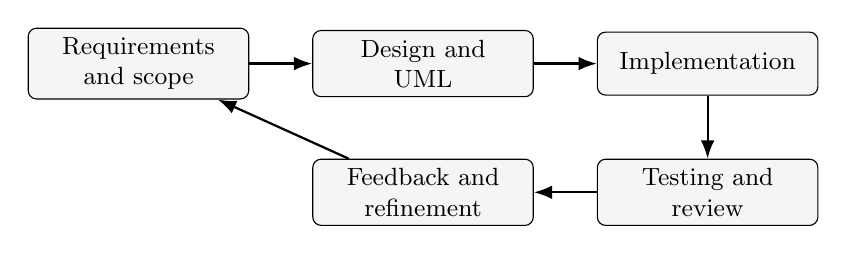
\begin{tikzpicture}[node distance=8mm,small]
\node[box] (req) {Requirements\\and scope};
\node[box,right=of req] (design) {Design and\\UML};
\node[box,right=of design] (impl) {Implementation};
\node[box,below=of impl] (test) {Testing and\\review};
\node[box,left=of test] (feedback) {Feedback and\\refinement};
\draw[arrow] (req)--(design); \draw[arrow] (design)--(impl); \draw[arrow] (impl)--(test); \draw[arrow] (test)--(feedback); \draw[arrow] (feedback)--(req);
\end{tikzpicture}
\caption{Iterative SDLC adopted for the project.}
\end{figure}

\section{System Architecture}
ReplayDB uses Next.js 15 with TypeScript and React for the user interface and API routes. The API layer exposes ledger, history, replay, transaction, and branch operations. In PostgreSQL mode, PL/pgSQL triggers capture row mutations into \texttt{replaydb.replay\_events}. In standalone mode, a deterministic in-memory ledger provides the same demonstration workflow without a database installation.

\begin{figure}[h]
\centering
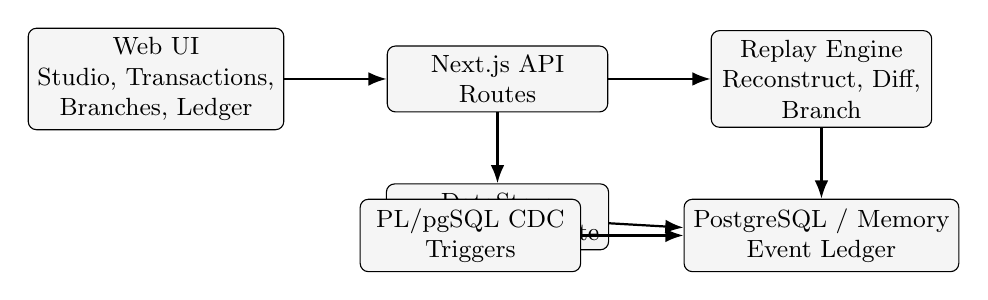
\begin{tikzpicture}[node distance=9mm and 13mm,small]
\node[box] (ui) {Web UI\\Studio, Transactions,\\Branches, Ledger};
\node[box,right=of ui] (api) {Next.js API\\Routes};
\node[box,right=of api] (engine) {Replay Engine\\Reconstruct, Diff,\\Branch};
\node[box,below=of api] (store) {DataStore\\shared demo state};
\node[box,below=of engine] (pg) {PostgreSQL / Memory\\Event Ledger};
\node[box,left=of pg] (trigger) {PL/pgSQL CDC\\Triggers};
\draw[arrow] (ui)--(api); \draw[arrow] (api)--(engine); \draw[arrow] (api)--(store); \draw[arrow] (engine)--(pg); \draw[arrow] (store)--(pg); \draw[arrow] (trigger)--(pg);
\end{tikzpicture}
\caption{High-level ReplayDB architecture.}
\end{figure}

\section{Class Diagram}
\begin{figure}[h]
\centering
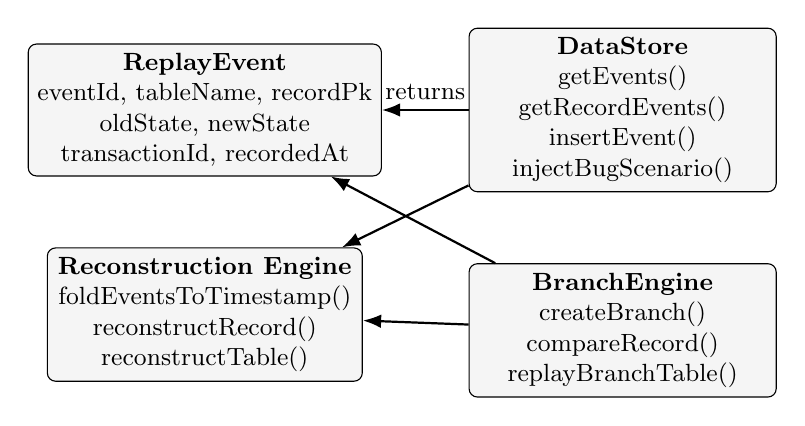
\begin{tikzpicture}[node distance=9mm and 11mm,small]
\node[box,minimum width=40mm] (event) {\textbf{ReplayEvent}\\eventId, tableName, recordPk\\oldState, newState\\transactionId, recordedAt};
\node[box,minimum width=39mm,right=of event] (store) {\textbf{DataStore}\\getEvents()\\getRecordEvents()\\insertEvent()\\injectBugScenario()};
\node[box,minimum width=39mm,below=of store] (branch) {\textbf{BranchEngine}\\createBranch()\\compareRecord()\\replayBranchTable()};
\node[box,minimum width=40mm,below=of event] (recon) {\textbf{Reconstruction Engine}\\foldEventsToTimestamp()\\reconstructRecord()\\reconstructTable()};
\draw[arrow] (store)--node[above]{returns}(event); \draw[arrow] (store)--(recon); \draw[arrow] (branch)--(recon); \draw[arrow] (branch)--(event);
\end{tikzpicture}
\caption{Core classes and their responsibilities.}
\end{figure}

\section{Activity Diagram: Incident Investigation}
\begin{figure}[h]
\centering
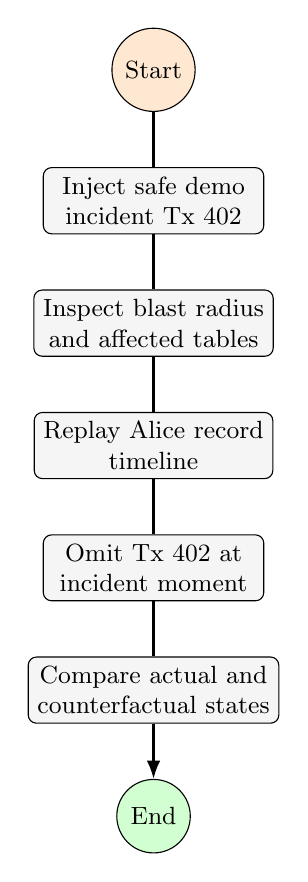
\begin{tikzpicture}[node distance=7mm,small]
\node[draw,circle,fill=orange!18,minimum size=7mm] (start) {Start};
\node[box,below=of start] (inject) {Inject safe demo\\incident Tx 402};
\node[box,below=of inject] (inspect) {Inspect blast radius\\and affected tables};
\node[box,below=of inspect] (replay) {Replay Alice record\\timeline};
\node[box,below=of replay] (branch) {Omit Tx 402 at\\incident moment};
\node[box,below=of branch] (compare) {Compare actual and\\counterfactual states};
\node[draw,circle,fill=green!18,minimum size=7mm,below=of compare] (end) {End};
\draw[arrow] (start)--(inject)--(inspect)--(replay)--(branch)--(compare)--(end);
\end{tikzpicture}
\caption{Activity flow for the guided incident investigation.}
\end{figure}

\section{Technology Stack}
\begin{itemize}
\item Front end: Next.js 15, React 19, TypeScript, Tailwind CSS, and Lucide icons.
\item Back end: Next.js route handlers and a TypeScript replay engine.
\item Database: PostgreSQL-compatible event capture using PL/pgSQL triggers; deterministic memory mode for demos.
\item Testing: Vitest unit and integration tests, API verification, responsive visual inspection, and end-to-end scenario testing.
\end{itemize}

\chapter{Implementation}
\section{Immutable Event Ledger}
Each mutation is represented as a \texttt{ReplayEvent}. It stores the record identity, operation type, old and new JSON states, transaction ID, timestamp, database user, and query context. These fields provide the evidence needed to explain a data change rather than merely display a final value.

\section{Replay Studio}
Replay Studio is the main investigative workspace. The user selects a table and record primary key, views the ordered event timeline, scrubs to a historical point, and reads the reconstructed row state. The field-diff tab highlights attributes changed by the selected mutation.

\section{Transaction Forensics and Counterfactual Branches}
The transaction page groups all events sharing a transaction ID. In the demo, Tx 402 changes the \texttt{users} and \texttt{accounts} tables, making the cross-table side effect visible as one atomic blast radius. A branch stores a name, base time, and excluded transaction IDs. The branch engine reconstructs the selected record with and without the excluded transaction and lists recovered fields side-by-side.

\section{Usability Improvements}
Visual testing led to a mobile navigation menu, a guided three-step incident workflow, clear error and retry feedback, and incident-moment branch comparison. These changes make the purpose of each page understandable to a first-time user.

\chapter{Testing and Evaluation}
\section{Testing Methodology}
Testing was performed at four levels: unit tests for reconstruction and diff algorithms, integration tests for API routes and feature interactions, manual API scenario checks, and browser-based end-to-end visual testing at desktop and mobile widths.

\begin{center}
\begin{tabular}{p{0.30\textwidth}p{0.36\textwidth}p{0.18\textwidth}}
\toprule
Test case & Expected result & Status \\
\midrule
Unit and integration suite & Core algorithms and API behaviours remain correct & 31/31 passed \\
Inject Tx 402 & Transaction is stored with two affected operations & Passed \\
Transaction forensics & Users and accounts mutations are shown together & Passed \\
Counterfactual branch & Tx 402 omitted: FRAUD/-5000 becomes ACTIVE/950.01 & Passed \\
Responsive navigation & Every product page remains reachable on mobile & Passed \\
Baseline reset & Demo returns to 7 events across 4 monitored tables & Passed \\
\bottomrule
\end{tabular}
\end{center}

\section{Evaluation Scenario and Results}
The main scenario begins with Alice's account active with a balance of 950.01. A simulated rogue batch transaction, Tx 402, sets the balance to -5000 and changes the status to FRAUD. Transaction Forensics identifies two affected rows: the user record and the related account record, which is frozen. Branch comparison omits Tx 402 at its incident time and recovers Alice's active status and original balance. The project therefore links an incorrect record to its causal transaction and demonstrates a read-only alternative state.

\chapter{Conclusion and Future Work}
\section{Summary of Work}
ReplayDB delivers a working temporal database debugging workflow. It combines change capture, event history, deterministic replay, field-level differences, transaction correlation, and counterfactual comparison in one browser interface.

\section{Key Findings and Future Work}
A usable forensic tool must make its state clear. Showing a raw log is insufficient; the selected record, time, transaction, affected tables, and comparison outcome must be connected in one flow. Future extensions include persistent PostgreSQL deployment, access control, pagination for large ledgers, richer correlation analysis, asynchronous replay, schema-evolution support, and exportable forensic reports.

\begin{thebibliography}{9}
\bibitem{nextjs} Vercel, \emph{Next.js Documentation}. Available: \url{https://nextjs.org/docs}.
\bibitem{postgres} PostgreSQL Global Development Group, \emph{PostgreSQL Documentation}. Available: \url{https://www.postgresql.org/docs/}.
\bibitem{course} TIET UCS503, \emph{Semester Project Guidance}. Available: \url{https://tiet-ucs503.github.io/semester-project/}.
\bibitem{vitest} Vitest, \emph{Vitest Documentation}. Available: \url{https://vitest.dev/}.
\end{thebibliography}

\end{document}
